\documentclass[__main__.tex]{subfiles}

\begin{document}

\section{Спектральный признак устойчивости с неявной разностной схемой для одномерного гиперболического уравнения}

Рассмотрим задачу Коши:

\begin{equation} \label{35.1}
\begin{cases}
\frac{\partial^2 U}{\partial t^2} - \frac{\partial^2 U}{\partial x^2} = 0, \ \left(x,t\right) \in \mathbb{R} \times \left(0,T\right) \\
U \left(x,0\right) = \varphi \left(x\right), \ \frac{\partial U}{\partial t} \left(x,0\right) = \psi \left(x\right), \ x\in \mathbb{R}
\end{cases}
\end{equation}

Конечно-разностную схему рассмотрим на сетке:

$$
C = A \times B = \langle \left(x_k, t^n\right) = \left(k h; n t\right): k \in \mathbb{Z}, n = \overline{0,N} \rangle
$$

Конечно-разностный аналог, аппроксимирующий задачу, создаётся с помощью $C$ - сеточной функции; заданный на слое n времени в виде: $U^n_{\left(\cdot\right)} = \left(U^n_k \in\mathbb{R}\right)_{\mathbb{Z}}$ в виде (неявная схема):

\begin{figure}[ht]
	\centering
	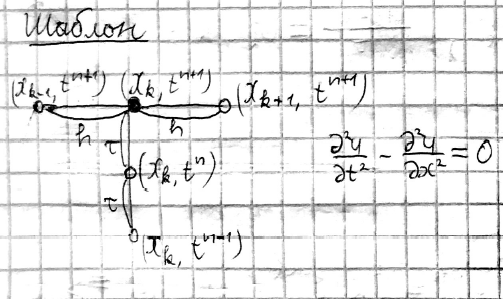
\includegraphics[width=0.4\linewidth]{img/img_35_1}
	\caption{}
	\label{img_34.1}
\end{figure}

\begin{equation}\label{35.2}
\begin{cases}
\frac{U^{n+1}_k - 2U^n_k+U^{n-1}_k}{\tau^2} - \frac{U^{n+1}_{k-1} -2U^{n+1}_k+U^{n+1}_{k+1}}{h^2} = 0 \\
\text{\ae} = \frac{\tau}{h} - \text{параметр Куранта}, \ k\in\mathbb{Z}, \ n = \overline{1,N-1}
\end{cases}
\end{equation}

\paragraph{Спектральный признак}
$$
\begin{cases}
U^{n-1}_k = e^{i \alpha k}$, $U^n_k = \lambda\left(\alpha\right) \cdot e^{i \alpha k}$, $U^{n+1}_k = \lambda^2 \left(\alpha\right) e^{i \alpha k}, \ k\in\mathbb{Z} \\
\end{cases}
$$.

Из (35.2) получаем:

$$
\lambda^2 \cdot e^{i\alpha k} - 2 \lambda \cdot e^{i\alpha k} + e^{i\alpha k} - \text{\ae}^2 \lambda^2 \cdot (e^{i\alpha (k+1)} -2e^{i\alpha k} + e^{i\alpha (k-1)}) = 0
$$

$$
\lambda^2 - 2 \lambda +1 - \text{\ae}^2 \lambda^2 (e^{i\alpha - 2 +e^{-i\alpha}})= 0
$$

$$
\lambda^2 (1 + 4 \text{\ae}^2 \sin^2 \frac{\alpha}{2}) + 2 \lambda +1 = 0
$$

$$
d = 1 - (1 - 4 \text{\ae}^2 \sin^2 \frac{\alpha}{2}) = - 4 \text{\ae}^2 \sin^2 \frac{\alpha}{2} 
$$

\paragraph{} 
	$\lambda =  $$\frac{1 \pm \sqrt{- 4 \text{\ae}^2 \sin^2 \frac{\alpha}{2}}}{1 + 4 \text{\ae}^2 \sin \frac{\alpha}{2}}$$ = $$\frac{1 \pm 2i \text{\ae} \sin \frac{\alpha}}{1 + 4 \text{\ae}^2 \sin^2 \frac{\alpha}{2}}$$$
	 
	$
	|\lambda| = \frac{1}{1 + 4 \text{\ae}^2 \sin^2 \frac{\alpha}{2}} \leq 1 \Rightarrow \text{устойчива}
	$

\end{document}
